\documentclass[10pt,twocolumn]{article}
\usepackage[letterpaper,margin=0.75in,columnsep=0.28in]{geometry}
\usepackage{times}
\usepackage[T1]{fontenc}
\usepackage{microtype}
\usepackage{amsmath,amssymb,amsthm}
\usepackage{graphicx}
\usepackage{booktabs}
\usepackage{multirow}
\usepackage[font=small,labelfont=bf]{caption}
\usepackage{xcolor}
\usepackage[numbers,sort&compress]{natbib}
\usepackage{enumitem}
\usepackage[colorlinks=true,linkcolor=blue!50!black,citecolor=blue!50!black,urlcolor=blue!50!black]{hyperref}
\setlist{nosep,leftmargin=*}
\newtheorem{proposition}{Proposition}
\graphicspath{{../figures/}}
\newcommand{\crc}{\textsc{crc}}

\title{\vspace{-0.6in}\bf Trust That Survives Deployment:\\Shift-Robust Review Guarantees for AI Medical Scribes}
\author{Kishore Nuthalapati\\{\small Independent researcher}\\{\small Code and data: \url{https://github.com/kishoren18-hue/scribecheck}}}
\date{\small Preprint, November 2026}

\begin{document}
\maketitle

\begin{abstract}
AI medical scribes write clinical notes from doctor--patient conversations, and their safety rests on a clinician reviewing each note. Conformal risk control (\crc) can tell that reviewer which sentences to check while bounding the expected share of errors left unflagged, but the bound assumes the notes at deployment are exchangeable with the notes used to calibrate it. A scribe deployment breaks that assumption: vendors update models, microphones change the transcript, and a hospital's cases differ from any benchmark. We build \textbf{ScribeErr}, 11,996 corrupted notes from ACI-Bench and MTS-Dialog with eleven transcript-aware error types, including \emph{grounded} errors whose every word was spoken during the visit. We find that (i) in distribution, \crc{} meets its 10\% target while missing 26.5\% of grounded errors, mostly negation flips; (ii) a vendor whose errors skew toward subtle types pushes the realized miss rate to 15.5\%, violating the target in 97\% of 300 resplits, whereas transcript noise leaves it valid but raises reviewer workload from 28\% to 41\% of sentences. We propose \textbf{type-conditional review guarantees}, which bound the miss rate within each error family and therefore under any mixture of families, and a \textbf{label-free shift alarm} built on bias-corrected label-shift estimation. Type-conditional \crc{} never exceeded a 1.6\% miss rate across six deployment conditions, but its price is set by the worst-detected family (80\% workload, driven by negation). Applying it only when the alarm fires keeps the miss rate at or below 2.5\% under every shift at 30\% workload when nothing has shifted. Finally, on 1,200 notes from ten real note writers, transcript checks with 93\% adjudicated precision find an invented drug, dose or side in 15\% of GPT-4 notes against 1.7\% of human notes, and a transcript-to-note certainty audit finds models stating hedged diagnoses as certain where human notes did not.
\end{abstract}

\section{Introduction}
Health systems are adopting ambient AI scribes faster than they can evaluate them. The assumed safety valve is the signing clinician, yet a recent audit of three commercial scribes found a verified failure in about one note in three, including a mode that no published taxonomy covered: a treatment the clinician retracted, recorded as delivered care~\citep{fox2026census}. Reviewers need to know which sentences to read.

Conformal risk control~\citep{angelopoulos2022crc} gives a principled answer. CARE~\citep{bedi2026care} applies it to medical summaries, flagging sentences so that the risk of an unflagged hallucination stays below a target across random resplits. Like every conformal method, the guarantee is marginal over exchangeable data. A deployed scribe violates exchangeability in at least three ways: the vendor's \emph{error mix} changes with model updates, \emph{transcript quality} changes with microphones and accents, and the \emph{case mix} changes between hospitals. A separate line of work shows that language models systematically inflate the certainty of clinical statements~\citep{du2026possible,belem2026may}, but neither study examines the conversation-to-note setting of a scribe.

We ask whether a review guarantee survives deployment, and what it costs to make one that does. Our contributions:
\begin{enumerate}
\item \textbf{ScribeErr}, a transcript-aware error benchmark separating \emph{grounded} errors (all words spoken, meaning wrong) from ungrounded ones, with retraction and negation types and real paired ASR transcripts (\S\ref{sec:bench}).
\item To our knowledge, the first stress test of \crc{} review guarantees under scribe-deployment shift, showing that error-mix shift breaks them and transcript noise inflates their cost (\S\ref{sec:results}).
\item \textbf{Type-conditional review guarantees} that hold under any error mix without deployment labels, a trust dial between marginal and type-conditional guarantees, and the empirical finding that their price is set by the worst-detected error family (\S\ref{sec:robust}).
\item A \textbf{label-free shift alarm} and an alarm-gated policy that pays for robustness only when the alarm fires, plus negation-aware evidence features that lower that price (\S\ref{sec:robust}).
\item A verified report card on 1,200 real notes from ten note writers and a transcript-to-note certainty audit (\S\ref{sec:real}).
\end{enumerate}

\section{The ScribeErr benchmark}\label{sec:bench}
\textbf{Sources.} ACI-Bench~\citep{yim2023aci} pairs 207 role-played visits with full notes; its virtscribe subset provides both a human transcription and a raw ASR transcript of the same audio for 28 test encounters. MTS-Dialog~\citep{benabacha2023mts} pairs shorter dialogues with single note sections and serves as an unseen corpus. Detectors are trained only on the 87 ACI-Bench train and validation encounters.

\textbf{Corruption.} Each instance leaves a reference note clean with probability 0.2 and otherwise injects one to four errors, each checked against the transcript (Table~\ref{tab:types}). Retractions use disjoint phrasing sets for training and testing. Severity is assigned by rule; 57\% of injected test errors are major.

\begin{table}[t]
\centering\small
\caption{ScribeErr error types and families.}\label{tab:types}
\setlength{\tabcolsep}{4pt}
\begin{tabular}{@{}lll@{}}
\toprule
Type & Change & Family \\
\midrule
U\_DOSE & dose never said & invented \\
U\_NUM & vital/lab/duration never said & invented \\
U\_MED & same-class drug never mentioned & invented \\
U\_LAT & side flipped, one side discussed & invented \\
U\_TIME & time unit shifted & invented \\
U\_FAB & fabricated symptom sentence & invented \\
NEG\_FLIP & polarity reversed & negation$^\dagger$ \\
G\_NUM & number said elsewhere in visit & grounded \\
G\_MED & drug discussed elsewhere in visit & grounded \\
G\_LAT & side flipped, both sides discussed & grounded \\
RETRACT & clinician retracts a recorded plan & grounded \\
\multicolumn{3}{@{}l}{\footnotesize $^\dagger$All words spoken; counted as grounded in \S4.} \\
\bottomrule
\end{tabular}
\end{table}

\textbf{Splits and shifts.} Training has 1,740 notes (60,980 sentences); the test set crosses 120 encounters, 5 seeds, 3 error mixes and 5 simulated ASR rates (9,000 notes, 322,530 sentences); the paired real-ASR set has 560 notes and MTS-Dialog 696. The \emph{uniform} mix weights types equally (42\% grounded); a \emph{subtle vendor} mix models a mature scribe that rarely invents facts but mis-binds and misses retractions (82\% grounded); a \emph{crude vendor} mix mostly invents (12\% grounded). Simulated ASR noise over-weights sound-alike drugs, teen/ty confusions and dropped laterality.

\section{Auditor and review gates}\label{sec:method}
\textbf{Evidence features.} For each note sentence the auditor computes about 40 features against the transcript: TF-IDF retrieval of the best three-turn window; unsupported content words, numbers, drugs and symptoms; dose-to-drug binding; laterality in the matched window; window polarity including doctor-question/patient-answer pairs; and, in the +R variant, whether a drug's last mention was a stop or hold turn. Gradient-boosted trees (SC) are trained on ScribeErr-train.

\textbf{Marginal \crc.} A sentence is flagged when its score is at least $\lambda$. For a note with errors, the loss is the fraction left unflagged; a note without errors has loss 0. \crc{} picks the largest $\lambda$ with $(n\hat R(\lambda)+1)/(n+1)\le\alpha$, which bounds the expected loss on an exchangeable new note. We also evaluate a severity-weighted version, a Hoeffding high-probability version (\crc-HP, $\delta=0.1$) and a stratified version.

\textbf{Protocol.} In each resplit, half of the 120 test encounters calibrate on the uniform, clean-transcript condition; gates are evaluated on held-out encounters under each shift (MTS-Dialog uses all its dialogues). We use $\alpha=0.10$ throughout.

\section{Results: the guarantee under shift}\label{sec:results}
\textbf{Detection.} Lexical grounding, the heuristic most auditors use, reaches AUROC 0.587 and falls below chance on grounded types. SC reaches 0.905 (calibrated ECE 0.002) but, against clean sentences from the same section and drug/number stratum, only 0.69 on negation flips and 0.71 on grounded numbers (Figure~\ref{fig:detector}).

\begin{figure*}[t]
\centering
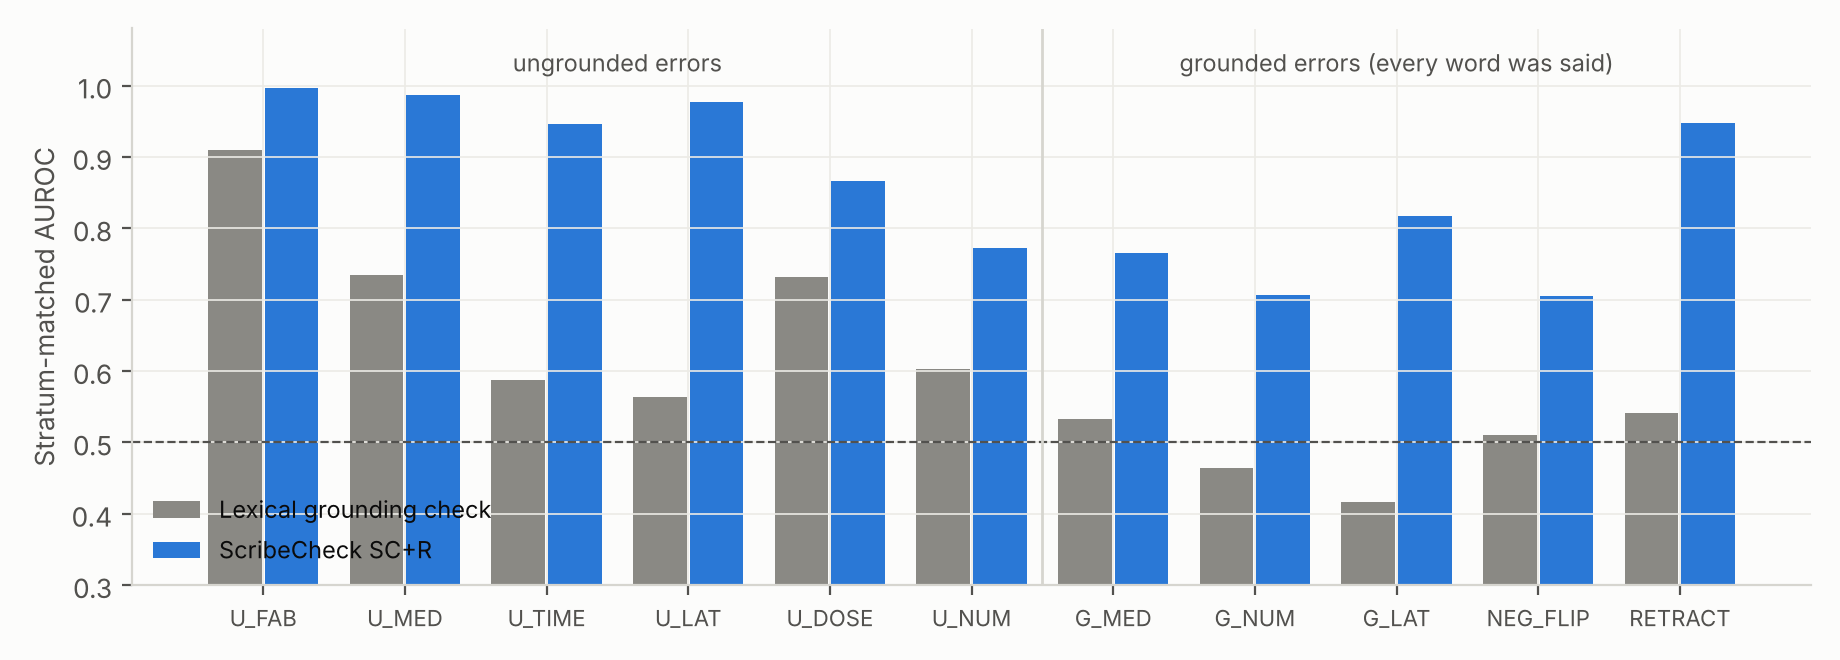
\includegraphics[width=0.78\textwidth]{fig2_detector_by_type.png}
\caption{Stratum-matched AUROC by error type. Lexical grounding is at or below chance on every grounded type.}\label{fig:detector}
\end{figure*}

\begin{table*}[t]
\centering\small
\caption{Marginal \crc{} and \crc-HP under deployment shift (SC auditor, $\alpha=0.10$, 300 resplits). Bold: target violated on average.}\label{tab:shift}
\begin{tabular}{@{}lccccc@{}}
\toprule
Deployment & \crc{} miss & P(miss$>\alpha$) & \crc{} workload & \crc-HP miss & \crc-HP workload\\
\midrule
In distribution & 0.098 & 0.44 & 28\% & 0.040 & 52\%\\
Simulated ASR 10\% / 30\% & 0.094 / 0.085 & 0.34 / 0.22 & 30\% / 35\% & 0.040 / 0.041 & 54\% / 57\%\\
Real ASR (paired) & 0.078 & 0.24 & 41\% & 0.005 & 91\%\\
New corpus (MTS-Dialog) & \textbf{0.107} & 0.79 & 36\% & 0.029 & 62\%\\
Crude vendor & 0.023 & 0.00 & 28\% & 0.008 & 52\%\\
Subtle vendor & \textbf{0.155} & 0.97 & 28\% & 0.055 & 52\%\\
Subtle vendor + ASR 20\% & \textbf{0.136} & 0.91 & 31\% & 0.046 & 55\%\\
\bottomrule
\end{tabular}
\end{table*}

\textbf{Two shifts, opposite effects.} Transcript noise makes clean sentences look less supported, so more cross the threshold: the miss rate falls and reviewer workload rises (28\% to 41\% on real ASR). Error-mix shift leaves clean scores unchanged but confronts the gate with the errors it scores lowest; a subtle vendor pushes the miss rate 55\% over target (Table~\ref{tab:shift}).

\textbf{A valid average hides who is missed.} In distribution \crc{} misses 26.5\% of grounded errors and 0.4\% of ungrounded ones. Negation flips are 32\% of grounded errors but about three-quarters of grounded misses (61\% missed); grounded sides 28\%, grounded numbers 16\%.

\textbf{Local repair.} Recalibrating on $m\approx80$ labeled site notes restores the target (0.091--0.094) at 40\% workload; \crc-HP holds everywhere without local labels at 52--62\% workload.

\section{Guarantees that survive error-mix shift}\label{sec:robust}
\textbf{Type-conditional \crc.} Partition errors into families $g\in\{$invented, negation, grounded$\}$. For each family run the conformal correction on that family's calibration errors, $\lambda_g=\max\{\lambda:(n_g\,\widehat{\mathrm{miss}}_g(\lambda)+1)/(n_g+1)\le\alpha\}$, and flag with $\lambda=\min_g\lambda_g$.

\begin{proposition}
Assume label shift across error families: the deployment distribution of auditor scores within each family equals the calibration distribution, and calibration errors within a family are exchangeable with deployment errors of that family. Then for any deployment family proportions $\pi$, the expected share of errors left unflagged is at most $\alpha$.
\end{proposition}
\begin{proof}[Sketch]
Each $\lambda_g$ satisfies the conformal bound for family $g$; because miss rates are non-decreasing in $\lambda$, $\mathrm{miss}_g(\lambda)\le\mathrm{miss}_g(\lambda_g)$, so $\mathbb E[\mathrm{miss}_g(\lambda)]\le\alpha$ for every $g$. The deployment miss rate is $\sum_g\pi_g\,\mathrm{miss}_g(\lambda)$, a convex combination.
\end{proof}
This is the label-conditional (Mondrian) construction~\citep{vovk2005algorithmic} applied to error families, related to conformal prediction under label shift~\citep{podkopaev2021label}; the guarantee is sentence-level, treating errors within a family as exchangeable. \textbf{The trust dial} MR-\crc($h$) interpolates: it guarantees every mix whose hard share (negation plus grounded) is at most $h$, requiring $(1-h)\,\mathrm{miss}_{\rm inv}+h\max(\mathrm{miss}_{\rm neg},\mathrm{miss}_{\rm gr})\le\alpha$ with finite-sample corrections.

\textbf{Label-free shift alarm.} A four-way family classifier trained on ScribeErr-train scores deployment sentences; its probabilities are bias-corrected on the labeled calibration notes by vector scaling, and deployment family proportions are re-estimated from unlabeled notes by expectation maximization~\citep{saerens2002adjusting,alexandari2020maximum}. With no shift the estimated hard share is 0.44 (true 0.42); for the subtle vendor 0.83 (true 0.82). Transcript noise biases the mix estimate but roughly doubles the estimated error rate, so the alarm fires when either signal leaves its in-distribution range (each threshold at the 97.5th percentile of in-distribution draws). The \textbf{alarm-gated policy} runs marginal \crc{} and switches to type-conditional \crc{} when the alarm fires.

\begin{table*}[t]
\centering\small
\caption{Mix-robust gates (SC auditor, $\alpha=0.10$, 200 resplits): mean miss rate / reviewer workload. Bold: target violated on average.}\label{tab:robust}
\begin{tabular}{@{}lcccccc@{}}
\toprule
Gate & No shift & Crude vendor & ASR 20\% & Subtle vendor & Subtle + ASR & New corpus\\
\midrule
\crc{} (marginal) & 0.100 / 28\% & 0.023 / 28\% & 0.091 / 32\% & \textbf{0.158} / 27\% & \textbf{0.138} / 31\% & \textbf{0.109} / 36\%\\
Trust dial, $h=0.4$ & 0.030 / 60\% & 0.005 / 60\% & 0.031 / 62\% & 0.044 / 59\% & 0.035 / 62\% & 0.020 / 69\%\\
Type-conditional \crc & 0.015 / 80\% & 0.000 / 80\% & 0.015 / 81\% & 0.016 / 80\% & 0.015 / 81\% & 0.002 / 84\%\\
Alarm-gated & 0.096 / 30\% & 0.023 / 29\% & 0.017 / 80\% & 0.025 / 78\% & 0.019 / 80\% & 0.002 / 84\%\\
\midrule
Alarm fire rate & 4.5\% & 1.5\% & 97.5\% & 94\% & 96.5\% & 100\%\\
\bottomrule
\end{tabular}
\end{table*}

\begin{figure*}[t]
\centering
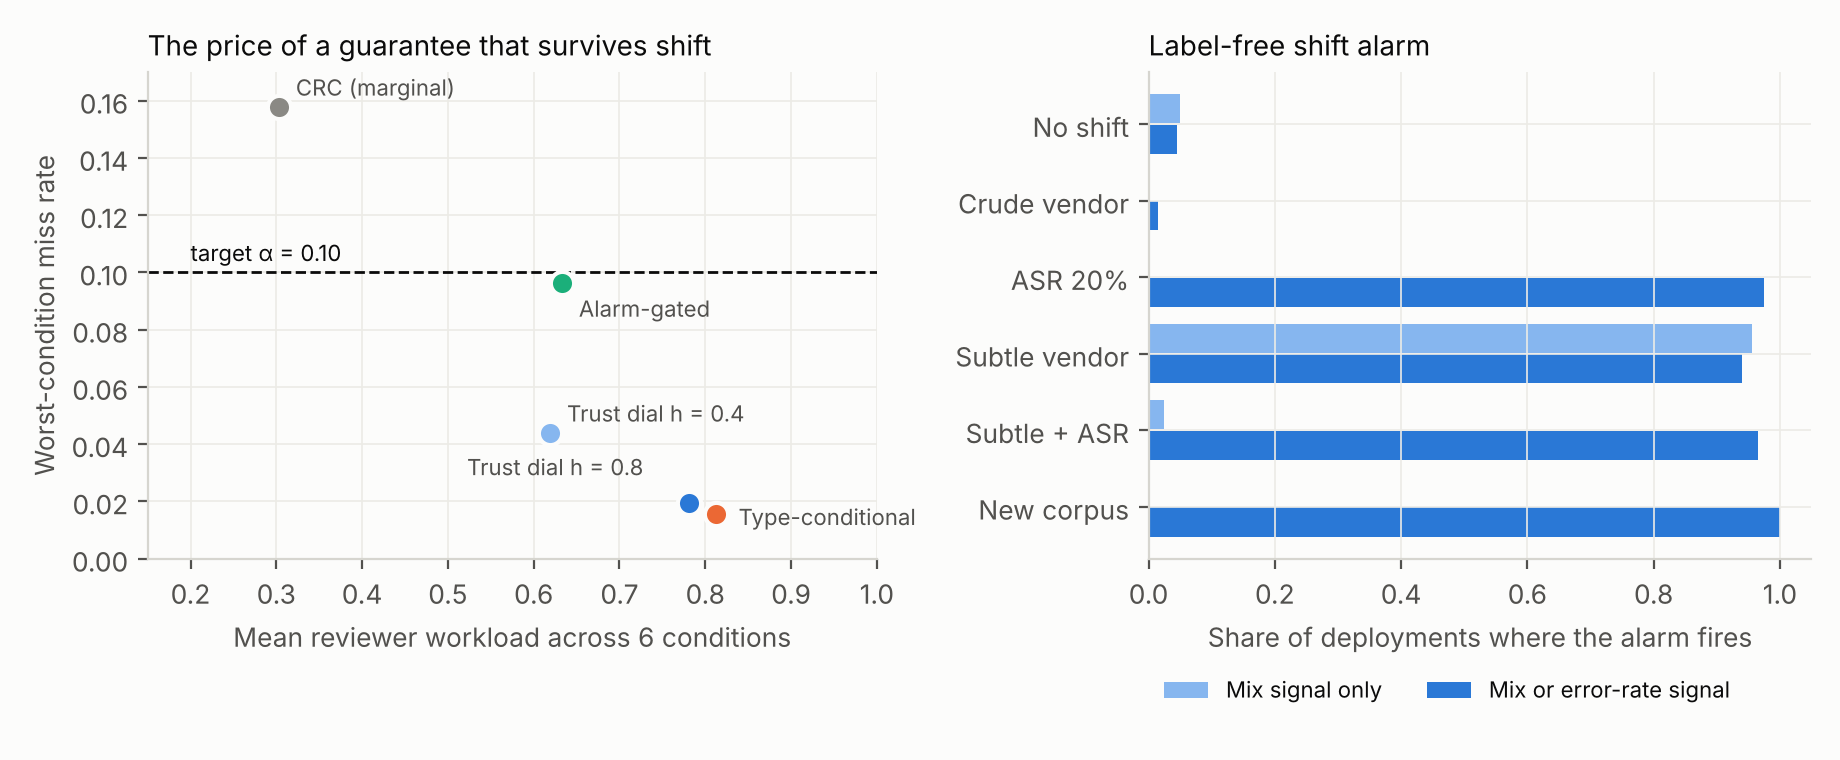
\includegraphics[width=0.86\textwidth]{fig7_mix_robust.png}
\caption{Left: mean reviewer workload against worst-condition miss rate. Right: share of deployments where the alarm fires.}\label{fig:robust}
\end{figure*}

\textbf{Results.} Type-conditional \crc{} and every trust-dial setting held the target in all six conditions and all 200 resplits, while marginal \crc{} failed in three conditions in 82--98\% of resplits (Table~\ref{tab:robust}, Figure~\ref{fig:robust}). The alarm-gated policy kept marginal \crc's cost when nothing shifted and the type-conditional guarantee under shift; its residual risk is the 6\% of subtle-vendor deployments where the alarm stayed silent.

\textbf{The price of trust is set by the worst-detected family.} Type-conditional \crc{} costs 80\% workload because negation flips are nearly invisible to the auditor. Dropping the negation family yields a type-conditional gate that costs the same as marginal \crc{} (29\%). Guaranteeing grounded binding errors is nearly free; guaranteeing negation is not.

\textbf{Negation-aware evidence.} We trace every clinical term in a note sentence to each visit turn that mentions it and score the mention as affirmed, denied (a negation cue before it, or a ``no'' answer to the doctor's question about it) or neutral, ignoring grammar so the auditor cannot learn injection artifacts. Negation detection rises from 0.69 to 0.74 stratum-matched AUROC; with retraction and polarity features combined, marginal \crc{} workload falls from 28\% to 22\% and type-conditional \crc{} from 80\% to 75\%, all guarantees intact.

\section{Report card on real note writers}\label{sec:real}
ACI-Bench released notes from nine systems for its 120 test encounters: GPT-4, ChatGPT, Text-Davinci-003 and -002 prompted zero-shot, and five fine-tuned summarizers. With the human reference notes these give ten writers on the same visits. These are 2023-era systems; the point is a protocol that grades any writer identically.

\textbf{Verified hard checks.} Four deterministic checks flag a drug never mentioned in the visit (brand and generic merged), a dose number never said, a dose said only for another drug, and a side stated when the visit names only the opposite side; transcript normalization handles spoken doses (``two point five'', ``seven and a half''). We adjudicated every flag on GPT-4 and human notes plus 41 sampled flags from other systems against the transcripts (82 flags): 68 genuine unsupported claims, 8 transcript mis-hearings (``57 twice a day'' for 750\,mg), 6 false alarms, for 93\% precision on unsupported content and 83\% on genuine note errors. \textbf{18 of 120 GPT-4 notes (15\%) contain a verified invented drug, dose or side, against 2 of 120 human notes (1.7\%).} Examples: a drug named when the patient said only ``the medication you prescribed''; ``Continue aspirin 81\,mg and clopidogrel 75\,mg'' in a visit that never mentioned antiplatelets; ``the high dose of atorvastatin'' rendered as 80\,mg. Low flag counts can reflect omission: the Davinci models record 52--72\% of the visit's drugs against 84\% for GPT-4 and 91\% for human notes (Table~\ref{tab:real}).

\textbf{Certainty audit.} For diagnoses the clinician hedged with a strong cue (``probably'', ``most likely'', ``rule out''), drawn from a fixed lexicon, we check whether the note's diagnostic sentences keep a hedge, state the diagnosis as certain, or omit it. Three validation rounds shaped the rules; after the last, every \emph{stated as certain} case among usable writers (7 of 7) was correct on reading. ACI-Bench yields only 23 such diagnoses in 22 visits, so this is a pilot: human notes kept all 16 hedges they recorded, Davinci-002 stated 3 of 12 as certain and ChatGPT 2 of 11 (``most likely due to rotator cuff tendinopathy'' became ``the doctor diagnosed \ldots{} rotator cuff tendinopathy'').

\begin{table}[t]
\centering\small
\setlength{\tabcolsep}{3.5pt}
\caption{Real note writers on 120 ACI-Bench visits. Flags: sentences with a hard-check flag (verified count in parentheses where all were adjudicated). Hedges: hedged diagnoses kept / stated certain / omitted.}\label{tab:real}
\begin{tabular}{@{}lcccc@{}}
\toprule
Writer & Sent./note & Drug cov. & Flags & Hedges\\
\midrule
Human reference & 35.7 & 0.91 & 12 (2) & 16/0/7\\
GPT-4 & 21.7 & 0.84 & 29 (26) & 13/1/9\\
ChatGPT & 13.7 & 0.66 & 1 & 9/2/12\\
Davinci-003 & 12.3 & 0.72 & 0 & 14/0/9\\
Davinci-002 & 11.2 & 0.52 & 0 & 9/3/11\\
BART-large & 12.9 & 0.46 & 17 & 0/0/23\\
BART-xsum-samsum & 12.5 & 0.46 & 12 & 0/0/23\\
BioBART & 11.9 & 0.41 & 14 & 0/1/22\\
LED & 5.6 & 0.46 & 93 & 6/2/15\\
LED-pubmed & 5.2 & 0.48 & 43 & 5/1/17\\
\bottomrule
\end{tabular}
\end{table}

\section{Limitations}
\textbf{Injected errors.} ScribeErr controls the error mix so shift can be studied; the subtle and crude mixes bracket plausible vendors without estimating any. Some injected negations read unnaturally; our negation features ignore grammar for this reason, but rates on natural errors may differ. \textbf{No clinician labels yet.} Adjudications were performed by the author against transcripts with AI assistance; a released labeling kit (blinded sheets, rubric, Krippendorff's $\alpha$) is the next step. \textbf{Assumptions.} Type-conditional guarantees assume label shift across families and treat within-family errors as exchangeable; transcript noise and new corpora violate the former, though the guarantee held empirically here. \textbf{Alarm.} The alarm missed 6\% of subtle-vendor deployments and its mix estimate is biased under noise. \textbf{Data.} Visits are role-played and real outputs come from 2023-era models; the certainty audit rests on 23 diagnoses. All guarantees are marginal or high-probability over calibration draws, never per note.

\section{Conclusion}
A review guarantee calibrated once can quietly stop holding when a scribe's error mix changes, and an average guarantee can hide the errors that matter. Bounding misses within each error family makes the guarantee robust to any mix, at a price set by the hardest family to detect, and a label-free alarm lets a deployer pay that price only when it is needed. The reviewer's question shifts from ``how often does the scribe err?'' to ``which errors am I guaranteed to see, and when has that stopped being true?''

\paragraph{Reproducibility.} All code, results, adjudication labels and figures: \url{https://github.com/kishoren18-hue/scribecheck}. \texttt{run\_all.sh} rebuilds every number from public data on two CPU cores with no API keys.

{\small
\bibliographystyle{plainnat}
\bibliography{refs}
}
\end{document}
